\section*{\bevezetes}

A beszámolóban ismertetem a szakmai gyakorlatom során végzett munkámat, bemutatásra kerül maga az Attrecto Zrt., ahol a gyakorlatomat végeztem, ismertetem a gyakornoki idő alatt rámbízott feladatokat, a kollégákat, akikkel együtt dolgoztam és a tapasztalataimat.
\par A következő fejezetekben először áttekintést nyújtok a vállalatról, majd ismertetem a szerepemet és a projekteket, amelyeken dolgoztam.

\section*{Attrecto Zrt.}
\begin{figure}[H]
    \centering
    \includegraphics[width= 100mm]{figures/Attrecto_logo.png}
\end{figure}
\par Az Attrecto Zrt-t 2010-ben alapította három fiatal győri szoftverfejlesztő. A cég megalakulása óta professzionális mobil- és webfejlesztést és tanácsadást nyújt az ország legnagyobb cégeinek, valamint az Egyesült Államokban, Norvégiában és Ausztráliában működő ügyfeleknek. 

\par A jelenleg 85 főt foglalkoztató vállalat 2021-ben mintegy 900 millió forint árbevételt ért el. A vállalkozások számára végzett frontend-fejlesztés a fő területük, de számos iparági céggel dolgoznak együtt. A cég alapítása óta Közép-Európában ismert vállalkozássá vált. Ismertségét nemzetközi piacokon elért sikerei is alátámasztják, mint például a norvég Telenor számára fejlesztett mobilalkalmazás, vagy az Egyesült Államokban régóta végzett munkájuk. A vállalat a Financial Times 1000 leggyorsabban növekvő vállalat listáján és a Deloitte Fast Tech 500 leggyorsabban növekvő európai technológiai vállalat listáján is szerepel.
\pagenumbering{gobble}

A legmodernebb technológiák felhasználásával készítik a legkorszerűbb alkalmazásokat és a hozzájuk kapcsolódó szerveroldali megoldásokat. Többnyire átláthatóan, rugalmasan és hatékonyan dolgoznak az agilis szoftverfejlesztési módszertan alkalmazásával, és ügyfeleiket digitális példaképpé formálják az adott iparágban.
\par A vállalat jó kapcsolatot ápol a győri Széchenyi István Egyetemmel, ahol évente kétszer négy technológiát felölelő gyakorlati foglalkozásokat szervez a hallgatóknak Attrecto Akadémia néven. A foglalkozások résztvevői egy gyakornoki program keretében ismerkedhetnek meg a vállalat működésével.
\par Avállalat szakmai élete belső szervezésű szakmai csoportokban, ún. szakmai Councilokban zajlanak. E csoportosulások a céges know-how management színterei, ahol rendszeresen van lehetőség az adott szakmai területhez tartozó tudásbázis fejlesztésére, valamint a tapasztalatcserére.
\section*{Angular keretrendszer}
\begin{figure}[H]
    \centering
    \includegraphics[width= 100mm]{figures/angular.png}
\end{figure}
Szakmai gyakorlatom során elsősorban az Angular frontend keretrendszerrel dolgoztam, amely egy TypeScript-alapú fejlesztési platform, amely a következőket tartalmazza:

\begin{itemize}
    \item Jól integrált könyvtárak gyűjteménye, amelyek a funkciók széles skáláját fedik le, beleértve az útválasztást, űrlapkezelést, ügyfél-kiszolgáló kommunikációt és még sok mást.
    \item Komponensalapú keretrendszer skálázható webes alkalmazások építéséhez.
    \item Egy fejlesztői eszközkészlet, amely segít a kód fejlesztésében, építésében, tesztelésében és frissítésében.
\end{itemize}
\par Az Angular egy front-end webfejlesztési keretrendszer, amelyet úgy terveztek, hogy megkönnyítse az egyoldalas alkalmazások (SPA-k) készítését. Alapja a TypeScript, a JavaScript egy szuperkészlete, és a Google tartja fenn. Az Angular deklaratív megközelítést használ, ami azt jelenti, hogy a fejlesztők megadják, hogy mit szeretnének az alkalmazással csinálni, az Angular pedig gondoskodik a mögöttes megvalósítás részleteiről.
\par Az Angular egyik legfontosabb jellemzője a komponensek használata, amelyek olyan moduláris kódblokkok, amelyek az alkalmazás egy adott részének sablonját (HTML) és logikáját (TypeScript) egyaránt tartalmazzák. A komponensek az egész alkalmazásban újrafelhasználhatók, ami megkönnyíti a nagyméretű alkalmazások készítését és karbantartását.
\par Az Angular emellett a webalkalmazások építéséhez gazdag funkciókészletet biztosít, többek között támogatja az adatkötést, a függőségi injektálást és a beépített direktívák átfogó készletét. Emellett tartalmaz egy nagy teljesítményű útválasztót is, amely lehetővé teszi a fejlesztők számára, hogy SPA-kat építsenek mély összekapcsolással és gazdag, interaktív élményekkel.
\par Összességében az Angular népszerű választás modern, interaktív webes alkalmazások építéséhez, és a fejlesztők világszerte széles körben használják.
\section*{A fejlesztés során használt szoftverek}
A szakmai gyakorlat első részében meg kellett ismerkednem a keretrendszerrel és a HTML, CSS és TS  eszközökkel, amelyek fontosak az Angular keretrendszer használatához. 
\par A mentoraimtól kaptam utasításokat a technológiák alapszintű elsajátítására, ez a tanulási folyamat körülbelül két hetet vett igénybe. A tanulási folyamat során megismertem a vállalatot, a mentorokat, a többi munkatársat és a munkafolyamatot.
\par A több hetes képzés során megismerkedtem a GitLab weboldalával és magával a Git verziókezelővel, valamint a Jira, Confluence és hasonló eszközökkel, amelyeket a vállalat a munkafolyamatok szervezésére és rögzítésére használ.
\par A következő bekezdésekben szeretném egy kicsit részletesebben is bemutatott a fent említett szoftvereket.
\subsection*{GitLab}
\begin{figure}[H]
    \centering
    \includegraphics[width= 90mm]{figures/gitlab.png}
\end{figure}
\par A GitLab egy webalapú Git-tárhelykezelő, amely verziókezelési, projektmenedzsment és folyamatos integrációs és telepítési (CI/CD) eszközöket biztosít. Arra tervezték, hogy segítse a csapatokat a szoftverfejlesztési projekteken való együttműködésben, és a teljes szoftverfejlesztési életciklus egy helyen történő kezelésében.
\par A GitLab segítségével a felhasználók Git-tárakat hozhatnak létre és kezelhetnek, nyomon követhetik és egyesíthetik a kódváltozásokat, valamint beépített eszközöket használhatnak a szoftver teszteléséhez, telepítéséhez és kiadásához. A GitLab számos projektmenedzsment- és együttműködési funkciót is biztosít, mint például a problémakövetés, a wikik és a csapatkommunikációs eszközök.
\par A GitLab elérhető saját üzemeltetésű és felhőalapú változatban is, és számos integrációt támogat más eszközökkel és szolgáltatásokkal. Sokféle szervezet használja, a kis startupoktól a nagyvállalatokig, számos iparágban.
\subsection*{Jira}
\begin{figure}[H]
    \centering
    \includegraphics[width= 90mm]{figures/Jira-Logo.png}
\end{figure}
\par A Jira szoftver egy projektmenedzsment eszköz, amely segít a csapatoknak a szoftverek tervezésében, nyomon követésében és kiadásában. Úgy tervezték, hogy támogassa az agilis módszertanokat, például a Scrumot és a Kanbant, és olyan funkciókat kínál, mint a testreszabható munkafolyamatok, a valós idejű jelentéskészítés és az integráció más eszközökkel. A Jira segítségével a csapatok nyomon követhetik és rangsorolhatják a munkát, együttműködhetnek a projektekben, és naprakészek maradhatnak a szoftverfejlesztés előrehaladásával kapcsolatban. A Jira-t különböző iparágak, köztük a szoftverfejlesztés, az informatika és a marketing területén működő szervezetek használják a projektek hatékony kezelésére és megvalósítására.
\subsection*{Confluence}
\begin{figure}[H]
    \centering
    \includegraphics[width= 90mm]{figures/Confluence.png}
\end{figure}
\par A Confluence az Atlassian által kifejlesztett csapatmunka- és dokumentációs szoftver. Arra tervezték, hogy segítse a csapatokat a tartalmak és információk létrehozásában, megosztásában és rendszerezésében egy központi helyen.
\par A Confluence segítségével a felhasználók dokumentumokat hozhatnak létre és szerkeszthetnek, valós időben együttműködhetnek a csapattagokkal, valamint nyomon követhetik a változásokat és a projekt előrehaladását. Emellett számos funkciót biztosít a tartalom szervezéséhez és strukturálásához, például sablonokat, címkéket és tereket.
\par A Confluence-t a kommunikáció és az együttműködés javítására széles körben használják a különböző iparágak csapatai, többek között a szoftverfejlesztés, a marketing, a pénzügy és az oktatás területén. Felhőalapú és helyhez kötött változatban is elérhető, és integrálható más eszközökkel és szolgáltatásokkal, például a Jira-val, a Slackkel és a Google Drive-val.
\subsection*{Movie App}
\par A több hetes tanulás végén egy bevezető feladatot kellett teljesítenem, egy egyszerű web alkalmazás formájában, amely filmborítókat jelenít meg, és részletesebb leírást ad róluk.
\par Ezt a webes alkalmazást természetesen az Angular keretrendszer segítségével kellett elkészítenem, és a fejlesztés során gyakorlatiasabb szempontból is megismerkedtem a fent említett eszközökkel és az Angular keretrendszerrel. A weboldal építése közben a mentorok a GitLab-on keresztül ellenőrizték a kódot, ahol magának a weboldalnak a kódját tartották számon. Minden fejlesztés külön kis ágként jött létre, amelyet ellenőriztek és merge requestként hozzáadtak a weboldal végleges kódjához.
\begin{figure}[H]
    \centering
    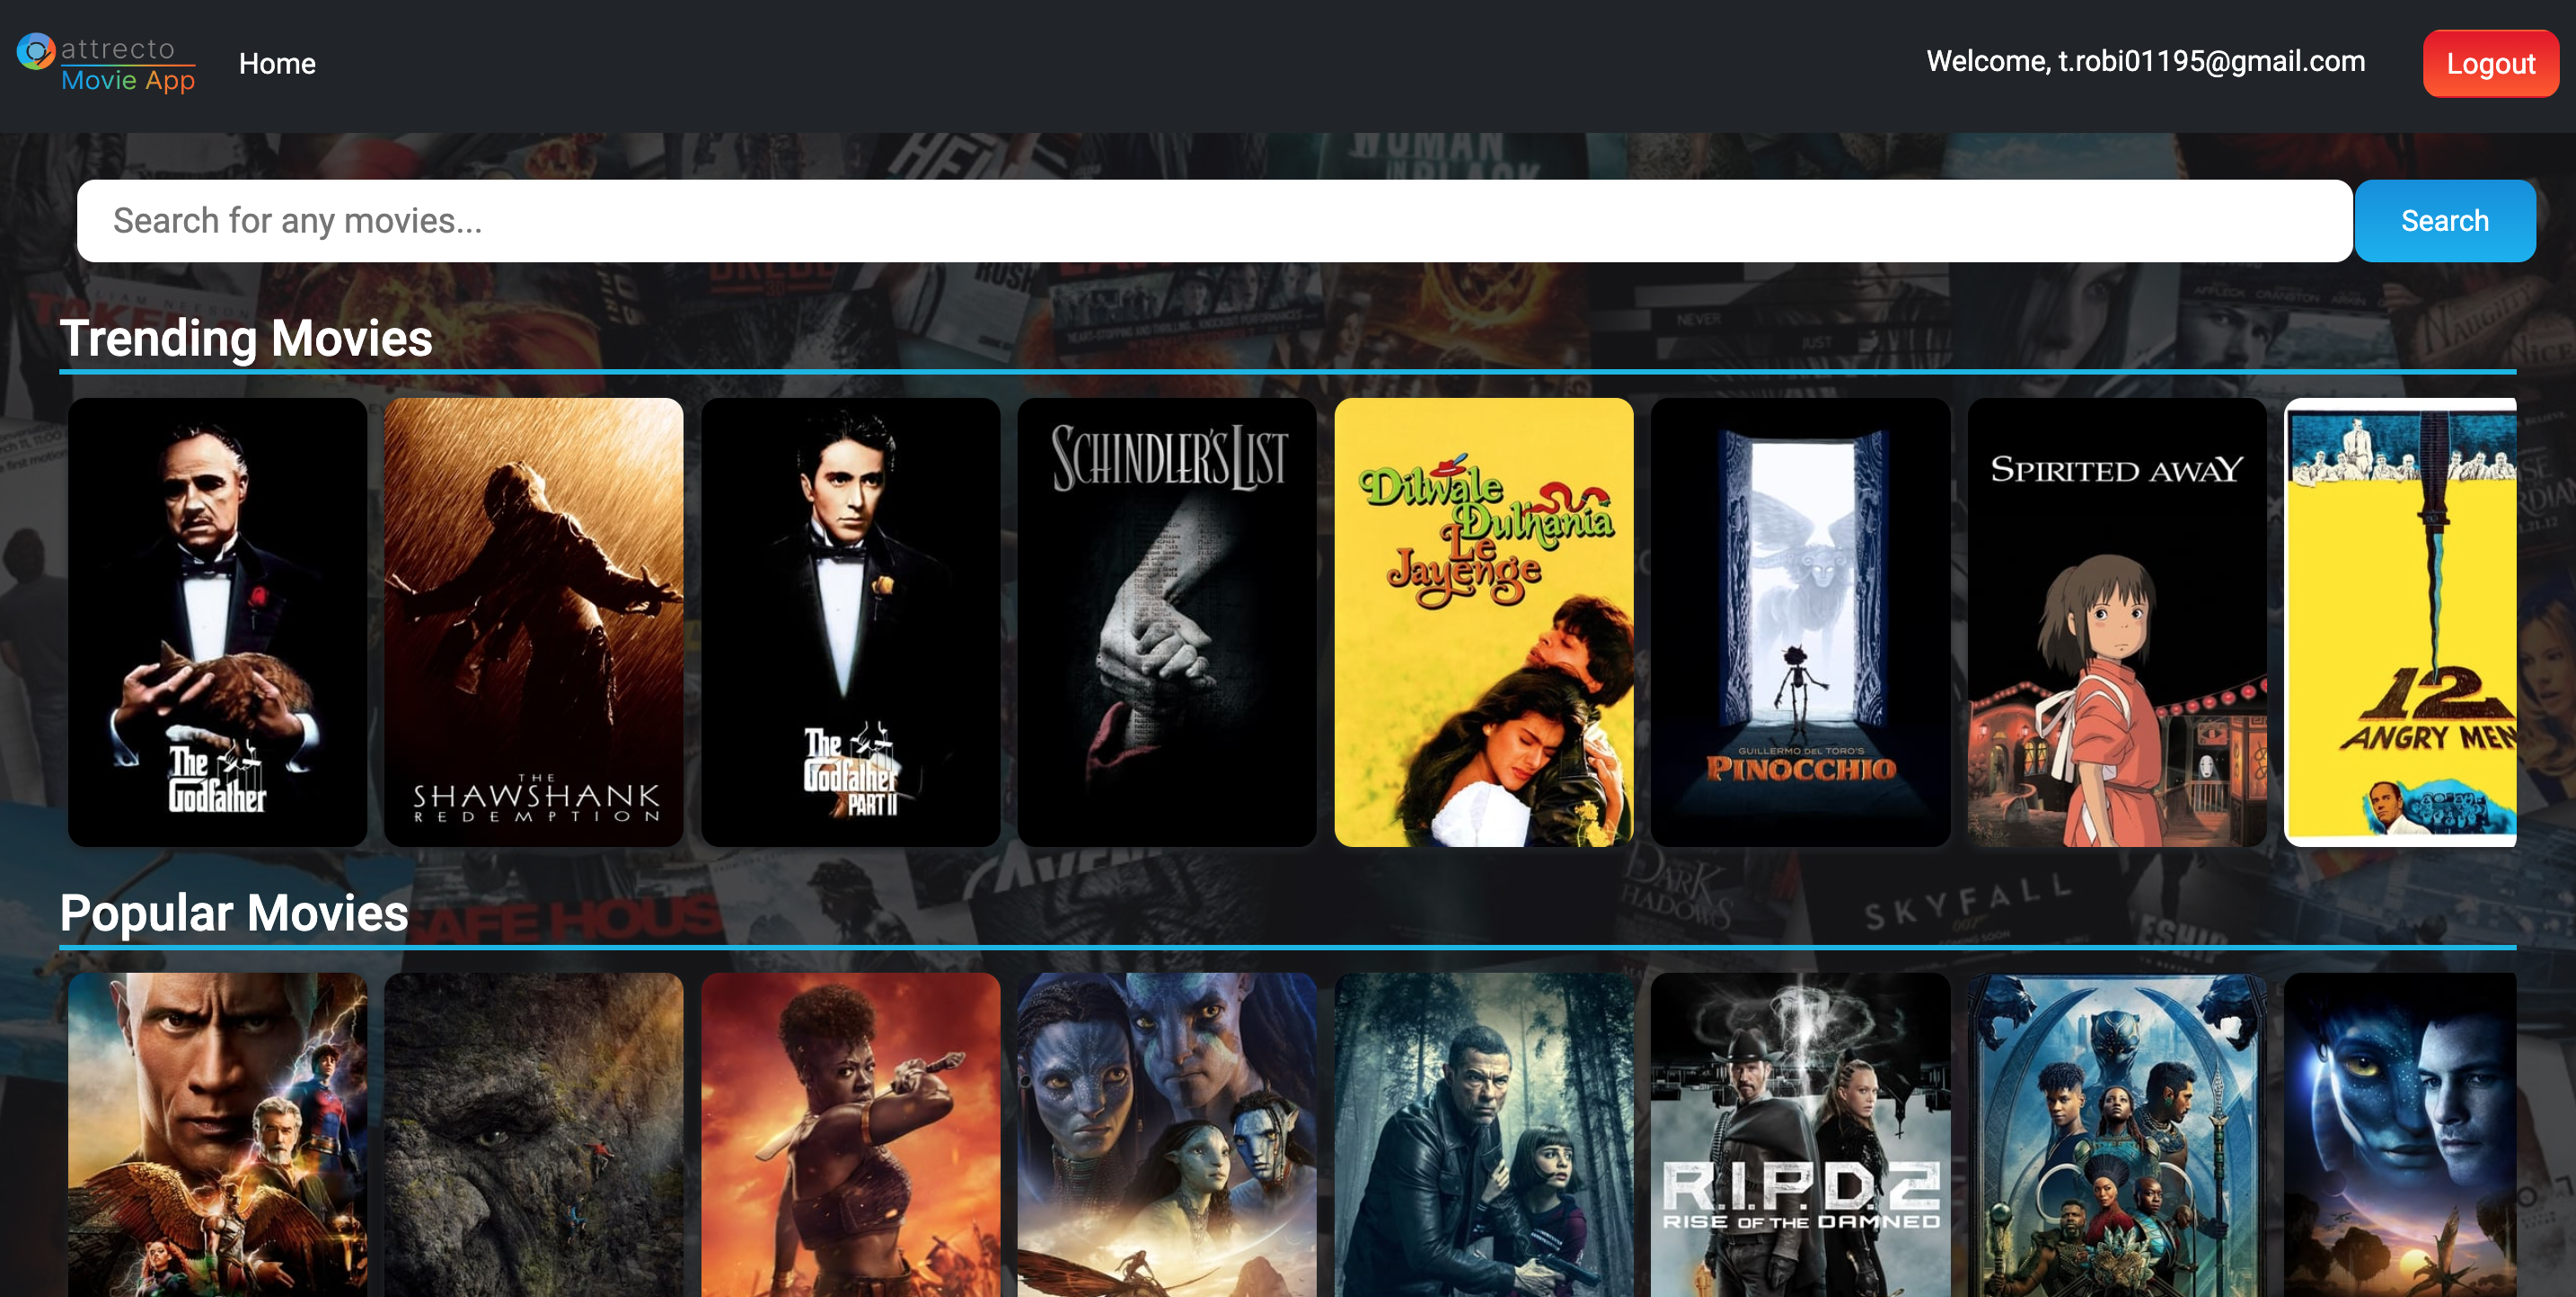
\includegraphics[width=140mm]{figures/movie-app.png}
    \captionsetup{labelformat=empty}
    \caption{Részlet a gyakornoki program feladatából}   
\end{figure}
\par A filmes gyakorlat után a többi gyakornokkal együtt részt vettem egy nagyobb projektben, ahol együtt dolgoztunk a vállalat belső weboldalának fejlesztésén. A fejlesztés sokkal nagyobb projekt volt, mint az előző gyakornoki alkalmak, ahol intenzíven használtam a Jira-t és a Confluence-t.
\par A projekt neve dashboard volt, amely egy olyan felület, amelyen a vállalat alkalmazottai különböző widgeteket helyezhetnek el tetszésük szerint. A webes alkalmazás Angular frontendre és több különböző backend technológiára (PHP, .NET stb.) épül, és mikrofrontend architektúrát használ minden egyes widgethez.
\par A kezdeti fázisokban a tervezés volt a fő hangsúly, a backend-fejlesztőkkel megbeszéléseket folytattunk a végpontokról és azok felépítéséről, majd a tervezés után elkezdtük az alkalmazás építését. Frontend oldalon az egyes feladatokat különböző widgetekre osztottuk, hogy könnyen, a fejlesztők közötti konfliktus nélkül fejleszthetőek legyenek.
\par A fejlesztés során az volt a feladatom, hogy létrehozzak néhány widgetet, miközben megtanultam a különböző könyvtárak használatát, a kódírást, a helyes programozási szokásokat és viselkedést, valamint a kód megfelelő formázását.
\section*{Összegzés}
\par Az Attrecto Zrt-nél töltött szakmai gyakorlatom során frontend fejlesztéssel foglalkoztam az Angular keretrendszer használatával, ahol megismerkedtem a HTML, JS és CSS technológiákkal, verziókezeléssel és projektmenedzsment eszközökkel. E munka során rengeteg tapasztalatot szereztem egy projekt lebonyolításának lépéseiről, valamint a kollégáimmal való kommunikációról és együttműködésről.
